\section{Existing DNU Tolerant Designs} \label{sec:DNUdes}

In this section, we discuss the existing DNU tolerant designs and give a background for the TNU latch. First we will discuss the DNU tolerant designs. The first proposed design, named the DNUCS latch and given in \cite{DNCS}, contains two DICE latches connected to a 2-input Muller C-element. An example of the C-element is given in Fig. \ref{HSMUF_fig}. The idea behind this design that it is impossible for a DNU to both DICE latches since they are SEU tolerant. More specifically, since the DICE latch is SEU tolerant, it requires a DNU to upset the data. The output Muller C-element only changes value when the inputs are unanimously the same value. Since both latches cannot be upset, the DNCS will tolerate a DNU. While this design is DNU tolerant, it is not DNU-robust since it may move to a high-impedance state after an error. 

Another design, named the interception latch and proposed in \cite{Inter}, improves on the DNCS by providing lower power consumption, delay and area. The latch functions using 6 two input Muller C-elements 

Currently, there are a few existing DNU tolerant designs. The first proposed design found in \cite{DNCS}, referred to as the DNCS latch, consists of two DICE cells connected to an output Muller C-element. This design tolerates DNU's since each DICE element requires a DNU to flip its state. Since the assumption is that only two errors can occur at once, in the worst case only one DICE element flips its state. Due to the C-element, the latch output does not change value. This design has been shown to be very resilient to DNUs at a very high cost of area, delay and power. The authors in \cite{Inter} propose an enhanced design compared to \cite{DNCS}. Their latch design consists of six 2 input C-elements connected in series which are then fed into a 3 input C-element. Like the DNCS latch, this design offers high resiliency to DNUs, however the power consumption and area overheads are still very high. 

More recently, a highly area and power efficient design has been proposed in \cite{HSMUF} and is referred to as the HSMUF latch. Fig. \ref{HSMUF_fig} provides the design. The HSMUF uses the TP-DICE \cite{TPDICE} structure which consists of 6 cross-coupled elements. In the case of a DNU, if the error is on an adjacent node (such as a strike on n1 and n2), the TP-DICE element will fully recover the previous state. However, if the strike occurs on two non-adjacent nodes, the TP-DICE will not fully recover leaving one output node with an erroneous value, one node at high impedance and the remaining output node held at the error-free value. To provide reliability, the three nodes are connected to a C-element, as in Fig. \ref{HSMUF_fig}, which allows the correct value to be held at the latch output. 

While all of the previously discussed designs do provide high DNU reliability, none of them are classified as DNU robust since a DNU will result in high impedance states on the internal and output nodes. If an error occurs after a DNU, these latch designs will flip their held value. A popular remedy to this issue is to place a weak keeper on the latch output as in Fig. \ref{HSMUF_fig}. However, adding a weak keeper greatly increases the power, area and delay overheads since the output C-element must be re-sized so that the C-element's driving strength exceeds that of the keeper. According to our simulations in Section \ref{sec:res}, the addition of the keeper to the HSMUF latch nearly triples the power consumption and delay. Additionally, the latch is still vulnerable to error after a DNU since the TP-DICE is in a high impedance state.

\begin{figure}[!htbp]
\centering
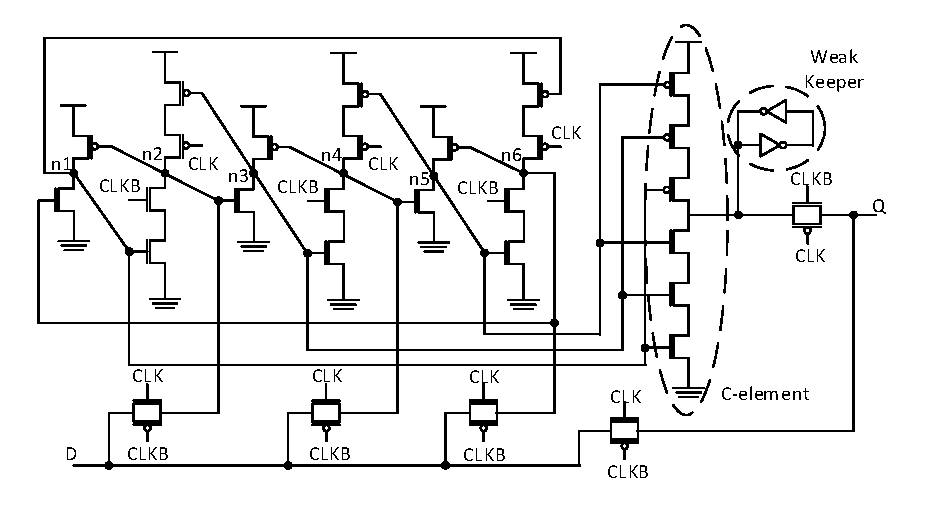
\includegraphics[width=\linewidth]{Figures/HSMUF}
 %where an .eps filename suffix will be assumed under latex, 
 %and a .pdf suffix will be assumed for pdflatex; or what has been declared
 %via \DeclareGraphicsExtensions.
\caption{HSMUF latch \cite{HSMUF} with a weak keeper on the output.}
\label{HSMUF_fig}
\end{figure}

To the author's knowledge, the existing most efficient DNU robust design capable of recovering all nodes after a DNU is the DONUT latch \cite{DONUT} in Fig \ref{fig:DONUT}. The design, as proposed in their paper, uses only 36 transistors but has a much higher power consumption compared to the HSMUF (See Section \ref{sec:res}). The reason for the high power consumption is due to contention on the input lines during the transparent mode. For example, if we observe node \textit{n2} in Fig. \ref{fig:DONUT} during the transparent mode, the node is driven by three cross-coupled elements. This contention will increase the amount of time required to change the node thus drastically increasing the dynamic power consumption. To optimize their design, we create the 48 transistor DONUT-M latch in which each component connected to an input node is modified, as shown in Fig. \ref{DONUT_M} so that the line is at high impedance for the whole duration of the transparent mode. This, in effect, removes the data contention problem thus reducing the overall dynamic power and delay.  

\begin{figure}[!htbp]
	\centering
	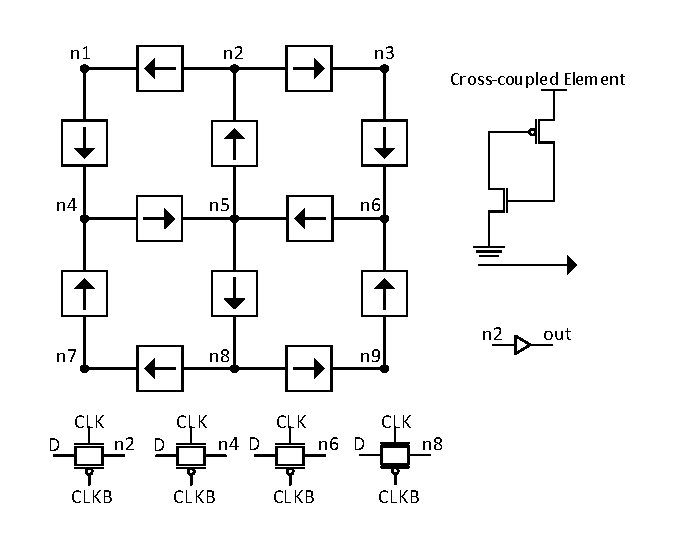
\includegraphics[width=\linewidth]{Figures/DONUT}
	%where an .eps filename suffix will be assumed under latex, 
	%and a .pdf suffix will be assumed for pdflatex; or what has been declared
	%via \DeclareGraphicsExtensions.
	\caption{DONUT latch as proposed in \cite{DONUT}.}
	\label{fig:DONUT}
\end{figure}

\begin{figure}[!htbp]
	\centering
	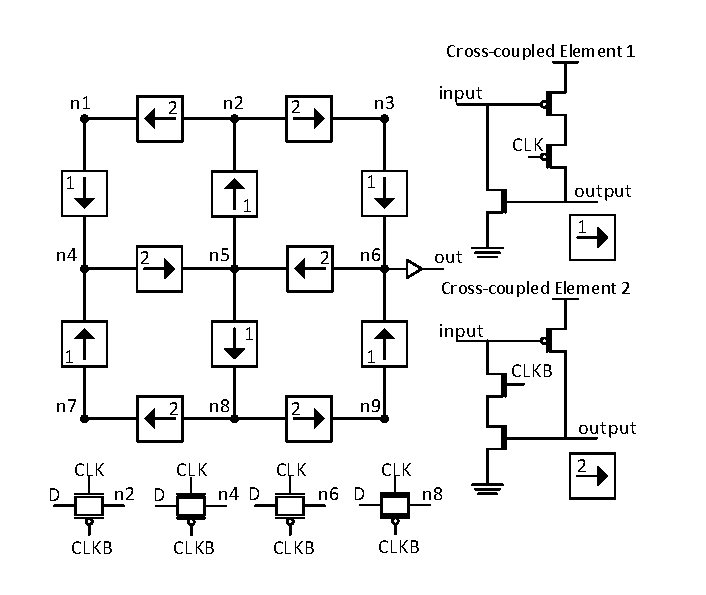
\includegraphics[width=\linewidth]{Figures/ModDONUT}
	%where an .eps filename suffix will be assumed under latex, 
	%and a .pdf suffix will be assumed for pdflatex; or what has been declared
	%via \DeclareGraphicsExtensions.
	\caption{Modified low-power DONUT latch.}
	\label{DONUT_M}
\end{figure}